\documentclass[12pt,a4paper]{article}
\usepackage{mwe}
\usepackage{tikz} 					% for drawing map
\usepackage{xcolor}					% for text color
\usepackage{amsthm} 				% Unnumbered theorem-like environments
\usepackage{hyperref}
\usepackage{enumitem}		 		% enumerate env
\usepackage{graphicx}				% insert img 
\usepackage{geometry} 				% page setups
\usepackage{titlesec}
\usepackage{tabularx,caption} 		% for table
\usepackage{mathtools, physics}		% math symbol & formula
\usetikzlibrary{mindmap}   			 % draw mindmap with tikz
\usepackage{amssymb}

\hypersetup{
	colorlinks=true,
	citecolor=black,
	filecolor=black,
	linkcolor=blue,
	urlcolor=blue
}
\geometry{
	a4paper,
	total={170mm,257mm},
	left=15mm,
	top=20mm,
}



% Set up one more sub level of section, then must redefine paragraph and subparagraph
\setcounter{secnumdepth}{4}
\titleclass{\subsubsubsection}{straight}[\subsection]
\newcounter{subsubsubsection}[subsubsection]

\titleformat{\subsubsubsection}
{\normalfont\normalsize\bfseries}
{\thesubsubsubsection}{1em}{}
\titlespacing{\subsubsubsection}
{0pt}{3.25ex plus 1ex minus .2ex}{1.5ex plus .2ex}

\makeatletter
\renewcommand\paragraph{\@startsection{paragraph}{5}{\z@}%
	{3.25ex \@plus1ex \@minus.2ex}%
	{-1em}%
	{\normalfont\normalsize\bfseries}}
\renewcommand\subparagraph{\@startsection{subparagraph}{6}{\parindent}%
	{3.25ex \@plus1ex \@minus .2ex}%
	{-1em}%
	{\normalfont\normalsize\bfseries}}

\def\toclevel@subsubsubsection{4}
\def\toclevel@paragraph{5}
\def\toclevel@paragraph{6}
\def\l@subsubsubsection{\@dottedtocline{4}{7em}{4em}}
\def\l@paragraph{\@dottedtocline{5}{10em}{5em}}
\def\l@subparagraph{\@dottedtocline{6}{14em}{6em}}
\makeatother

\setcounter{secnumdepth}{4} % how many sectioning levels to assign numbers to
\setcounter{tocdepth}{4} % how many sectioning levels to show in Table of Contents


% Renumber section
\renewcommand\thesection{\Alph{section}}
\renewcommand\thesubsection{\Roman{subsection}}
\renewcommand\thesubsubsection{\arabic{subsubsection}}
\renewcommand\thesubsubsubsection{\alph{subsubsubsection}}

% Trong's command
\newcommand{\img}[3]{
	\includegraphics[width=#1, height=#2]{{#3}}}	
\newcommand{\red}[1]{\textcolor{red}{\textbf{#1}}}
\newcommand{\blue}[1]{\textcolor{blue}{\textbf{#1}}}
\newcommand{\green}[1]{\textcolor{green}{\textbf{#1}}}
\newcommand{\titlePage}{
	\begin{titlepage}
		\centering
		
		{\huge \bfseries Mathematical note\par}
		\vspace{.5cm}
		{\Large Personal note\par}
		\vspace{.5cm}
		{\textsc{FPT University} \par}
		
		\vspace{2cm}
		{\Large\itshape Compiled by\par}
		\vspace{.5cm}
		{\textsc{Nguyễn Đức Trọng} \par}
		{\large November 7, 2022\par}
		
		\begin{flushright}
			{\textsc{Signature} \par}
			\img{2.5cm}{2.8cm}{Picture/Sign.png}
		\end{flushright}
	\end{titlepage}
}

% Math modes: inline math and display math
% Ex:
% a/ $\sum_{n=1}^{\infty} 2^{-n} = 1 $  -> inline math
% b/ \[\sum_{n=1}^{\infty} 2^{-n} = 1\] -> displat math -> more beautiful
% $...$ (more preferable) or \(...\) for inline math
% $$...$$ or \[...\] (more preferable) for display math
% \[...\] is a shorthand for displaymath env which is an un-numbered of equation env
% 
% Get space in Math mode
% \; - a thick space
% \: - a medium space
% \, - a thin space
% \! - a negative thin space

%%%%%%%%%%%%%%%%%%%%%%%%%%%%%%%%%%%%%%%%%%%%%%%%%%%%%%%
\newcommand{\superscript}[1]{^{{#1}}}
\newcommand{\subscript}[1]{_{{#1}}}

\def\arrowtext#1#2{\hbox to#1{\arrowtextA\ #2 \arrowtextA\kern2pt\llap{$\succ$}}}
\def\arrowtextA{\leaders\vrule height2.7pt depth-2.3pt\hfil}

\newcommand{\logab}[2]{\log_{#2} {#1}}
\newcommand{\xpower}[1]{x^{#1}}


\newtheorem*{definition}{Definition}
\newtheorem*{notation}{Notation}
\newtheorem{example}{Example}

\newcommand{\argmin}{\operatorname*{argmin}}
\newcommand{\argmax}{\operatorname*{argmax}}
%%%%%%%%%%%%%%%%%%%%%%%%%%%%%%%%%%%%%%%%%%%%%%%%%%%%%%%%%%%%%
%https://en.wikibooks.org/wiki/LaTeX/Mathematics

\begin{document}
\titlePage
\tableofcontents
\newpage


\section{Univariate Calculus}
\subsection{Overview}					% finished
\begin{tikzpicture}[grow cyclic, text width=2.7cm, align=flush center,
level 1/.style={level distance=8cm,sibling angle=20},]
%level 2/.style={level distance=2cm,sibling angle=45}
	\node{Function}
	child{node{Monotonicity}}
	child{node{Derivative}}
	child{node{Limit}}
	child{node{Inversion}}
	child{node{Composition vs Combination}}
	child{node{Transformation}}
	child{node{Evenness vs Oddity}}
	child{node{Categories}}
	child{node{Representation}}
	child{node{Definition}}
;	
\end{tikzpicture}

\subsection{Definition}					% finished
\noindent \textbf{Formal definition}: A function relates each element of a set with exactly one element of another set.\\ \\ \noindent

\noindent \textbf{Informal definition}: A specific calculation rule will yield what we want for inputs.\\ \\ \noindent
\textbf{Notation}:\\
f: X $\mapsto$ Y\\ \\ \noindent
\begin{figure}[h!]
\img{7cm}{2cm}{Picture/Univariate_calculus/Definition/1.png}
\caption{Machine diagram for a function f}
\end{figure}

\begin{figure}[h!]
\img{7cm}{6cm}{Picture/Univariate_calculus/Definition/2.png}
\caption{A mapping f from set D to set E}
\end{figure}
\newpage
\begin{figure}[h!]	\img{7cm}{6cm}{Picture/Univariate_calculus/Definition/3.png}
\caption{Some relevant terms}
\textbf{Notes}:\\
+ Function domain (tập xác định): What goes into the function.\\
+ Function range/ image (tập miền, ảnh): What is returned by the function.\\
+ Codomain: What may possibly come out from the function.\\
\end{figure}
\noindent
Examples:\\
a/ $y = f(x) = 5x + 7$\\
b/ $y = f(x) = 99x\superscript{2} + 100x + 9999 + 7\logab{5}{2}$\\ \\ \noindent
In practice,\\
+ The right hand side (RHS) is an independent variable or inputs.\\
+ The left hand side (LHS) is an dependent variable or outputs.\\
\subsection{Representations}			% finished
1/ Verbally (description)\\
2/ Numerically (table)\\
3/ Visually (graph)\\
4/ Algebraically (formula)\\

\subsection{Categories}					% Incomplete
There are several rudimentary functions we should bear in mind their properties.\\
\begin{tikzpicture}[grow cyclic, text width=2.7cm, align=flush center]
	\tikzstyle{level 1}=[level distance=4cm,sibling angle=180] 
	\tikzstyle{level 2}=[level distance=4cm,sibling angle=72]

	\node(root){Function}
	child{node{Algebraic}
		child{node{Polynomial func}}
		child{node{Power func}}
		child{node{Reciprocal func}}
		child{node{Rational func}}
	}
	child{node{Transcendental}
		child{node{Logarithmic func}}
		child{node{Exponential func}}
		child{node{Trigonometric func}}
		child{node{Periodic func}}
	}
;
\end{tikzpicture}
\subsubsection{Algebraic functions}
{\Large \textbf{Polynomial}}\\
A function f(x) is called a polynomial if
\begin{center}
$f(x) = a\subscript{n}x\superscript{n} + a\subscript{n-1}x\superscript{n-1} + a\subscript{n-2}x\superscript{n-2} + ... + a\subscript{1}x\superscript{1} + a\subscript{0}x\superscript{0}$
\end{center}
where:\\
+ n (>= 0): polynomial degree.\\
+ $a\subscript{0}, a\subscript{1}, a\subscript{2}$, ...: coefficients.\\
+ $a\subscript{n}$: leading coefficient.\\ \\ \noindent
Examples:\\
a/ $P(x) = 2\superscript{6} - x\superscript{4} + \frac{2}{5}x\superscript{3} + \sqrt{2}$\\
b/ $H(x) = x\superscript{4} + x\superscript{2} + 10$\\
\begin{figure}[h!]
\centering\img{7cm}{2cm}{Picture/Univariate_calculus/Categories/1.png}
\caption{Some graphs of polynomial function]}
\end{figure}
\newline
\noindent In polynomial function at a fundamental level, we pay more attention to \textbf{quadractic function} and \textbf{cubic function}.\\ \\ \noindent
\textbf{a/ Quadratic function}\\
General form:
\begin{center}
$f(x) = ax\superscript{2} + bx + c$
\end{center}
Solution formula:
\begin{center}
	$x = \frac{-b \pm \sqrt{\Delta}}{2a}$, where
	$\Delta = b\superscript{2} - 4ac = 0$
\end{center}
$\Delta$: Discriminant (định thức)\\
\textbf{Discriminant properties}:\\
+ $\Delta$ < 0: Function has no solution (vô nghiệm)\\
+ $\Delta$ = 0: Function has double root (nghiệm kép)\\
+ $\Delta$ > 0: Function has two distinct solutions (hai nghiệm p/b)\\ \\ \noindent
\textbf{Viète's formula for quadratic function} \vspace{1mm}\\
Sum of roots: $\Sigma = S = r\subscript{1} + r\subscript{2} = -\frac{b}{a}$ \vspace{3mm}\\
Product of roots: $\Pi = P = r\subscript{1}r\subscript{2} = \frac{c}{a}$\\
\vspace{1mm}\\
From $\Sigma$ and $\Pi$ we can establish the function via the Viète's formula:
\begin{center}
$f(x) = x\superscript{2} - Sx + P \Rightarrow x = \frac{S\pm\sqrt{S^{2} - 4P}}{2}$
\end{center}
\noindent \textbf{b/ Cubic function}\\
General form:
\begin{center}
$f(x) = ax\superscript{3} + bx\superscript{2} + cx + d = 0$\\
\end{center}
Solution formula: See at \href{https://www.wikihow.com/Solve-a-Cubic-Equation}{Wiki How}\\\\
\textbf{Viète's formula for cubic function} \vspace{1mm}\\
Sum of roots: $\Sigma = S = r\subscript{1} + r\subscript{2} + r\subscript{3}= -\frac{b}{a}$ \vspace{3mm}\\
Product of roots: $\Pi = P = r\subscript{1}r\subscript{2}r\subscript{3} = -\frac{d}{a}$ \vspace{3mm}\\
Pairwise sum of product:$r\subscript{1}r\subscript{2} + r\subscript{1}r\subscript{3} + r\subscript{2}r\subscript{3} = \frac{c}{a}$
\vspace{3mm}\\
Then applying substitution for find solutions.\\ \\ \noindent
{\Large \textbf{Power function}}\\
General form:
\begin{center}
$f(x) = x\superscript{a}$
\end{center}
where:\\
+ a = n or $\frac{1}{n}$ with n > 0 \vspace{1mm}\\
+ a = n or $\frac{1}{n}$ with n < 0

\begin{figure}[h!]
\centering\img{7cm}{4cm}{Picture/Univariate_calculus/Categories/2.png}
\caption{a = n with n > 0}
\centering\img{7cm}{4cm}{Picture/Univariate_calculus/Categories/3.png}
\caption{a = $\frac{1}{n}$ with n > 0}
\end{figure}

\newpage

\begin{figure}[h!]
\centering\img{6cm}{4cm}{Picture/Univariate_calculus/Categories/4.png}
\caption{a = -1}
\centering\img{6cm}{4cm}{Picture/Univariate_calculus/Categories/5.png}
\caption{a = -2}
\end{figure}

It is not finished yet.

\subsubsection{Transcendental functions}
\Large \textbf{Trigonometric Functions} \vspace{3mm}\\
\normalsize \indent In calculus, \textbf{radian} will be used in place of \textbf{degree}. Plus, trigonometric is one of the typical \textbf{periodic functions} that will be discussed in section.
\begin{figure}[h!]
\centering\img{10cm}{4cm}{Picture/Univariate_calculus/Categories/6.png}\caption{Graph of sin(x) and cos(x)}
\end{figure}
\newline
For more info, watch video from 79 $\rightarrow$ 108 in \hyperlink{https://youtube.com/playlist?list=PLDesaqWTN6ESsmwELdrzhcGiRhk5DjwLP}{Precalculus course}  of Professor Leonard

\noindent\Large \textbf{Periodic Functions}\\ 
\normalsize \indent Function that repeats itself in \textbf{regular intervals} or \textbf{periods}. Conversely, it is an aperiodic function.
\begin{center}
$f(x) = f(x + T)$, T is known beforehand
\end{center}
\textbf{Terminology}:\\
Consider in the form that: $f(x) = Acos(\omega t + \varphi)$\\
1/ Period - T: The length between two successive peaks\\
SI unit: s\\\\
2/ Frequency - $f$: How many peaks in one unit of time\\
SI unit: Hz\\\\
3/ Angular velocity - $\omega$: Time rate at which an object rotates, or revolves\\
SI unit: rad/$s^2$\\
Conversion formula: $\omega = 2\pi f = \frac{2\pi}{T}$\\\\
4/ Initial phase - $\varphi$: The initial function position on Ox\\
SI unit: radian\\\\
5/ Amplitude - A: The high of peak from the coordinate origin

Periodic functions have an intimate relationship with Fourier serier, Fourier transform, or Harmonic oscillation.



\subsection{Evenness vs Oddity}
\label{Evenness vs Oddity}
\Large \textbf{Odd function}

\normalsize \hspace{.5cm} A function such that $f(-x) = -f(x)$ over the domain of $f$.\\
Geometrically, $f(-x)$ is symmetry with respect to the origin (O)\\
Ex: $x$, $x^3$, and $sin(x)$
\begin{figure}[h!]
\caption{Graph of odd function}
\centering\img{3cm}{3cm}{Picture/Univariate_calculus/Oddity_Eveness/odd_1.png}
\end{figure}

\noindent \Large \textbf{Even function}

\normalsize \hspace{.5cm} A function such that $f(-x) = f(x)$ over the domain of $f$.\\
Geometrically, $f(-x)$ is symmetry with respect to y axis\\
Ex: $\frac{1}{x^2}$, $\abs{x}$, $x^3$, and $cos(x)$
\begin{figure}[h!]
\caption{Graph of even function}
\centering\img{3cm}{3cm}{Picture/Univariate_calculus/Oddity_Eveness/even_1.png}
\end{figure}

\noindent \Large \textbf{Properties}

\vspace{1mm}
\noindent\normalsize 1/ $f(x)=0$ satisfies both odd and even condition.\\\\
Additivity\\
2/ Even + Even = Even\\
3/ Odd + Odd = Odd\\\\
Multiplicity\\
4/ Even * Even = Even\\
5/ Odd * Odd = Even\\
6/ Odd * Even = Odd\\\\
Divisibility\\
7/ $\frac{Even}{Even} = Even$\\
8/ $\frac{Odd}{Odd} = Even$\\
9/ $\frac{Odd}{Even} = Odd$ $g(x)=\xpower{2}$)\\\\
Derivative\\
10/ $ \dv{x}$(Even) = Odd\\
11/ $ \dv{x}$(Odd) = Even\\\\
Composition\\
12/ $(Odd\circ Even)(x)$ = Even\\


\subsection{Transformation}
\subsection{Composition vs Combination}
\subsection{Inversion}
\subsection{Limit}
\subsection{Derivative}
\subsection{Monotonicity}



\section{Fourier series}
\subsection{Overview}					% finished
\begin{tikzpicture}[grow cyclic, text width=2.7cm, align=flush center]	
	\tikzstyle{level 1}=[level distance=3cm,sibling angle=90] 
	\tikzstyle{level 2}=[level distance=4cm,sibling angle=90]
	 
	\node(root){Fourier series}
	child{node{Series construction}
		child{node{test}}
	}
 	child{node{Preliminaries}
		child{node{Oddity \& Eveness}}
		child{node{Singularity Functions}}
	}
	
;
\end{tikzpicture}

\subsection{Preliminaries}					% Incomplete
\subsubsection{Function Oddity \& Eveness}
See at \hyperref[Evenness vs Oddity]{Evenness vs Oddity}
\subsubsection{Singularity functions}

\section{Linear Algebra}
\subsection{Overview}
Linear algebra is the way to organize and deal with a large set of number - matrix. Linear algebra is widely applied in almost AI fields from rudimentary to advanced topics. In addition, The combination between Linear algebra and Calculus leads to matrix calculus which will be discussed later.\\
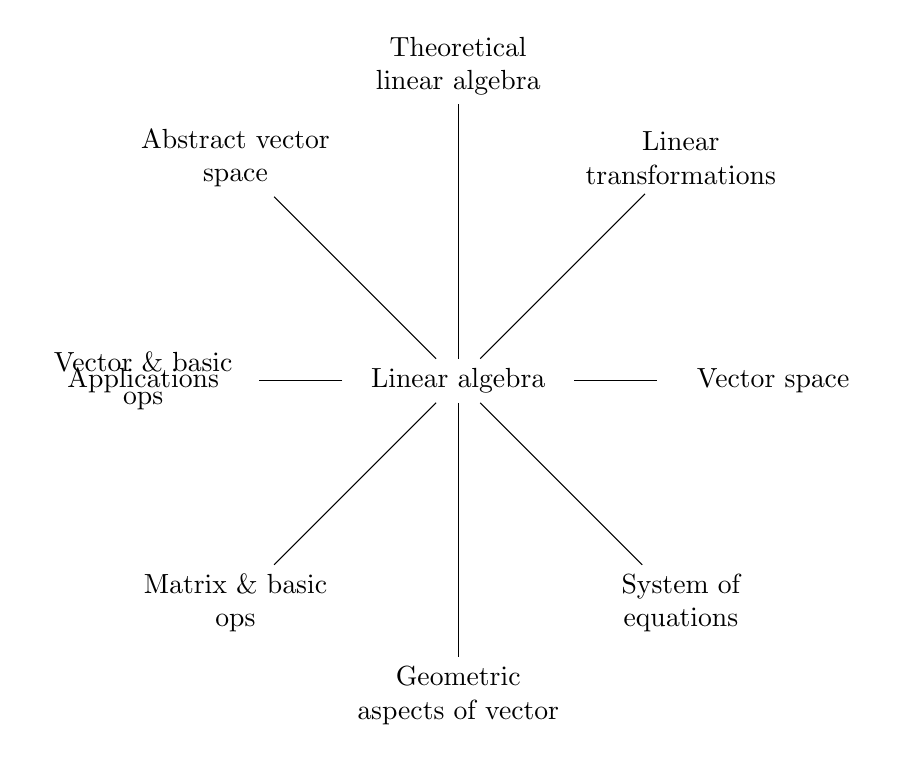
\begin{tikzpicture}[grow cyclic, text width=2.7cm, align=flush center]	
	\tikzstyle{level 1}=[level distance=4cm,sibling angle=45] 
	
	\node(root){Linear algebra}
	child{node{Vector \& basic ops}}
	child{node{Matrix \& basic ops}}
	child{node{Geometric aspects of vector}}
	child{node{System of equations}}
	child{node{Vector space}}
	child{node{Linear transformations}}
	child{node{Theoretical linear algebra}}
	child{node{Abstract vector space}}
	child{node{Applications}}
	;
\end{tikzpicture}

\subsection{Vector \& basic operations}
\textbf{Definition}: A vector $\vec{v}\in\mathbb{R}^{n}$ is an n-tuple of real numbers.\\

\noindent\textbf{Notation}\\
a/$\mqty[x_1& x_2& \hdots & x_n]$ for row vector\\\\
b/$\mqty[x_1\\ x_2\\ \vdots\\ x_n]$ for col vector\\
$x_1, x_2, x_3, ...$ are called components or coordinates of vector.\\
\noindent To derive a uniform for further formula, col vector is chosen as a representation for vector.\\

\noindent\textbf{Example}\\
a/$\vec{v}=\mqty[1\\ 2\\ \vdots\\ n]$ is a column vector in $\mathbb{R}^{n}$\\

\noindent\textbf{Basic vector operations}\\
+ Addition\\
+ Scaling\\
+ Subtraction (represented via addition and scaling)\\

\noindent\textbf{Example}\\
a/ \red{Addition}\\
Algeraic aspect\\
$\vec{v_1}=\mqty[1\\ 2\\ 3]$, $\vec{v_2}=\mqty[4\\ 5\\ 6]$\\
$\vec{v_3}=\vec{v_1}+\vec{v_2}=\mqty[1\\ 2\\ 3]+\mqty[4\\ 5\\ 6]=\mqty[5\\ 7\\ 9]$\\

\noindent Geometric aspect\\
\begin{figure}[h!]
\centering\img{10cm}{4cm}{Picture/Linear_algebra/Vector_and_basic_ops/1.png}
\caption{Addition of two vectors: the parallelogram rule}
\end{figure}

\noindent b/ \red{Subtraction}\\
Algeraic aspect\\
$\vec{v_1}=\mqty[4\\ 5\\ 6]$, $\vec{v_2}=\mqty[1\\ 2\\ 3]$\\
$\vec{v_3}=\vec{v_1}-\vec{v_2}=\mqty[4\\ 5\\ 6]-\mqty[1\\ 2\\ 3]=\mqty[3\\ 3\\ 3]$\\

\noindent Geometric aspect\\
\begin{figure}[h!]
\centering\img{6cm}{4cm}{Picture/Linear_algebra/Vector_and_basic_ops/2.png}
\caption{Subtraction of two vectors}
\end{figure}

\noindent c/ \red{Scailing}\\
Algeraic aspect\\
$\vec{v_1}=\mqty[1\\ 2\\ 3]$\\
$\vec{v_3}=3\vec{v_1}=3\mqty[1\\ 2\\ 3]=\mqty[3\\ 6\\ 9]$\\


%+ Scalar/ Dot product\\
%+ Cross product/ Directed area product/ Vector product\\
%+ Length/ L2 Norm\\
%+ Normalization\\
%
%
%
%
%\noindent d/ Dot product\\
%\begin{figure}[h!]
%\centering\img{6cm}{4cm}{Picture/Linear_algebra/Vector_and_basic_ops/3.png}
%\caption{Scalar product}
%\end{figure}
%
%\noindent e/ Cross product\\
%Algeraic aspect\\
%$v_1=\mqty[1\\ 2\\ 3]$, $v_2=\mqty[4\\ 5\\ 6]$\\
%$v_1\cross v_2=\mqty[\abs{\mqty{2&5\\ 3&6}}\\\\ -\abs{\mqty{1&4\\ 3&6}}\\\\ \abs{\mqty{1&4\\ 2&5}}]= \mqty[-3\\ 6\\ -3]$\\
%
%\noindent Geometric aspect\\
%\begin{figure}[h!]
%\centering\img{6cm}{4cm}{Picture/Linear_algebra/Vector_and_basic_ops/4.png}\\
%\centering\img{6cm}{4cm}{Picture/Linear_algebra/Vector_and_basic_ops/5.png}\\
%\centering\img{6cm}{4cm}{Picture/Linear_algebra/Vector_and_basic_ops/6.png}\\
%\caption{Scalar product}
%\end{figure}
%
%\noindent Length\\
%Algeraic aspect\\
%$v=\mqty[1\\ 2\\ 3]$\\
%$\abs{\abs{v}}=\sqrt{v.v}=r\sqrt{1^2+2^2+3^3}=$\\
%
%\noindent Geometric aspect\\
%
%
%\noindent h/ Normalization\\
%$v=\mqty[1\\ 2\\ 3]$\\
%$\hat{v}=\frac{v}{\abs{\abs{v}}}=\frac{1}{\sqrt{1^2+2^2+3^2}}\mqty[1\\ 2\\ 3]=\frac{1}{\sqrt{14}}\mqty[1\\ 2\\ 3]$

\subsection{Matrix \& basic ops}
Matrix can be interpreted in two different ways.\\
\indent $1^{st}$ way: A set of column vectors is put in adjacent order.\\
\indent $2^{nd}$ way: A way to represent coefficients of system of equations.\\

\noindent \textbf{First interpretation}\\
Assume that we have a contrived dataset as the following:\\
\begin{table}[h!]
	\begin{center}
		\begin{tabular}{l|l|l|l|l}
		Price  & Type          & Area & Location       &  \\
		1B\$   & Semi-detached & 400  & 10km to centre &  \\
		1.5B\$ & Single family & 700  & 20km to centre &  \\
		2B\$   & Multi-family  & 1000 & 50km to centre & 
		\end{tabular}
		\captionof{table}{Contrived dataset for housing price}
	\end{center}
\end{table}
\newline
from this dataset, the matrix will be
\begin{displaymath}
	\mqty[10^9& 0& 400 & 10\\
	1.5*10^9  & 1& 700 & 20\\
	2*10^9    & 2& 1000& 50\\]
\end{displaymath}


\noindent \textbf{Second intepretation}\\
Assume that we have a system of equations as the following:\\
\begin{displaymath}
\begin{cases}
	x+2y+3z=5\\
	2x+9y+10z=50\\
	3x+12y+15z=90\\
\end{cases}
\end{displaymath}
then the matrix will be
\begin{displaymath}
\left[
\begin{array}{ccc|c}
1&  2&   3& 5\\
2&  9&  10& 50\\
3&  12& 15& 90\\
\end{array}
\right]
\end{displaymath}
\textbf{Note}:\\
+ Uppercase for matrix name\\
+ Lowercase for matrix entry/ component\\

\noindent\textbf{Basic matrix operations}\\
+ Addition: $\mathbb{R}^{m\cross n}+\mathbb{R}^{m\cross n}=\mathbb{R}^{m\cross n}$\\
+ Subtraction: $\mathbb{R}^{m\cross n}-\mathbb{R}^{m\cross n}=\mathbb{R}^{m\cross n}$\\
+ Multiplication: $\mathbb{R}^{m\cross l}\cross\mathbb{R}^{l\cross n}=\mathbb{R}^{m\cross n}$\\

\noindent Addition and subtraction are performed as follows:\\
$C=A\pm B \iff c_{ij}=a_{ij}\pm b_{ij}, \forall i\in[1,...,m], \forall j\in[1,...,n]$\\

\noindent Matrix multiplication are performed as follows:\\
$C=AB \iff c_{ij}=\sum_{k=1}^{l} a_{ik}b_{kj}, \forall i\in[1,...,m], \forall j\in[1,...,n]$\\

\noindent \textbf{Example}\\
Suppose we have\\
$A=\mqty[1 & 2& 3\\
         4 & 5& 6]$
$B=\mqty[2 & 3& 4\\
		 5 & 6& 7]$
$C=\mqty[1 & 2\\
		 3 & 4\\
		 5 & 6\\
		 ]$\\\\
\noindent a/Addition\\
$D=A+B=
\mqty[1 & 2& 3\\ 4 & 5& 6]+
\mqty[2 & 3& 4\\ 5 & 6& 7]
=\mqty[1+2 & 2+3& 3+4\\ 4+5 & 5+6& 6+7]
=\mqty[3 & 5& 7\\ 9 & 11& 13]$\\
      
\noindent b/Multiplication\\
$E=AC=
\mqty[1& 2& 3\\
      4& 5& 6]
\mqty[1& 2\\
      3& 4\\
      5& 6]
=\mqty[1.1+2.3+3.5 & 1.2+2.4+3.6\\
       4.1+5.3+6.5 &4.2+5.4+6.6]
=\mqty[\admat{25& 28\\ 49& 64}]$\\
\textbf{Matrix taxonomy}\\
1/ Square matrix\\
Matrix has size/ dimension n by n
2/ Retangular matrix\\
Matrix has size/ dimension n by n
3/ Unit/ Identity matrix\\
All entries are 1\\

4/ Zero/ Null matrix\\
All entries are 0\\

5/ Diagonal matrix\\
Off-diagonal entries equals 0
6/ Upper triangular matrix\\
7/ Lower triangular matrix\\
\newpage
\section{Machine learning}
\subsection{Overview}	% finished
Machine learning is commonly split according to:\\
\indent+ Learning style\\
\indent+ Funtion-based algorithm\\
\indent+ Charactered-based algorithm\\
\noindent
According to the taxonomy in Artificial Intelligence A Modern Approach chapter 5, when mentioning about learning style, we have as following:\\
\begin{tikzpicture}[grow cyclic, text width=2.7cm, align=flush center]	
	\tikzstyle{level 1}=[level distance=4cm,sibling angle=120] 
	\tikzstyle{level 2}=[level distance=4cm,sibling angle=90]
	
	\node(root){Style}
	child{node{Supervised Learning}
		child{node{Classification}}
		child{node{Regression}}
	}
	child{node{Unsupervised Learning}
		child{node{Clustering}}
		child{node{Association}}
	}
	child{node{Reinforcement Learning}}
;
\end{tikzpicture}

In function-based algorithm, we will have:\\
\begin{tikzpicture}[grow cyclic, text width=2cm, align=flush center]
	\tikzstyle{level 1}=[level distance=7cm,sibling angle=52] 
	\tikzstyle{level 2}=[level distance=2.5cm,sibling angle=80]
	
	\node(root)[grow=down]{Function}
	child{node{Regression}
		child{node{OLS}}
		child{node{Logistic}}
		child{node{Stepwise}}
	}
	child{node{Classification}
		child{node{Decision tree}}
		child{node{SVM + variants}}
	}
	child{node{Clustering}
		child{node{k-Means}}
		child{node{k-Medians}}
		child{node{EM}}
	}
	child{node{Instance-based}
		child{node{kNN}}
		child{node{LVQ}}
	}
	child{node{Bayesian Algo}
		child{node{Naive Bayes}}
		child{node{Gaussian Naive Bayes}}
	}
	child{node{Dim Reduction}
		child{node{PCA}}
		child{node{LDA}}
	}
	child{node{Ensemble Methods}
		child{node{XGBoost}}
		child{node{AdaBoost}}
		child{node{Random Forest}}
	}
;
\end{tikzpicture}
With the last one, we will have:\\
In function-based algorithm, we will have:\\
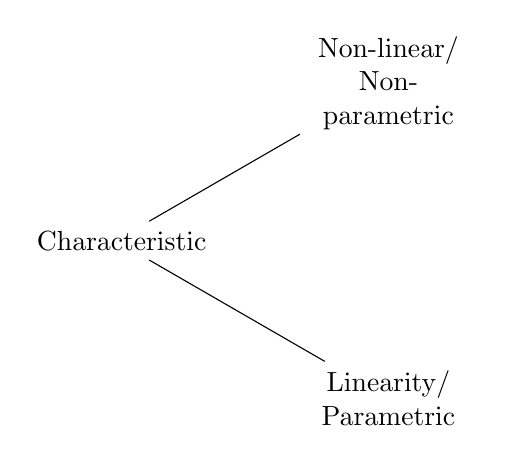
\begin{tikzpicture}[grow cyclic, text width=2cm, align=flush center]
	\tikzstyle{level 1}=[level distance=4cm,sibling angle=60] 
	
	\node(root)[grow=down]{Characteristic}
	child{node{Linearity/ Parametric}}
	child{node{Non-linear/ Non-parametric}}
;
\end{tikzpicture}
\subsection{Learning style}
\subsubsection{Supervised learning} % finished
Supervised learning (SVL) is applied when we want to make a prediction for a whole dataset and a set of desired labels/ patterns. We can think it as the following flow,\\
(Label, Data) \arrowtext{3.5cm}{SVL model} Trained model \arrowtext{5.5cm}{Predict with new data} What label of a new data is.\\

\noindent In mathematical lingo, we have:\\
Training dataset $\mathcal{X} = \{\mathbf{x}_1, \mathbf{x}_2, \dots, \mathbf{x}_N\}$ and label dataset $\mathcal{Y} = \{\mathbf{x}_1, \mathbf{x}_2, \dots, \mathbf{x}_N\}$, where $\mathcal{X} \& \mathcal{Y}$ are two attributes of a collected dataset. Then we want to make a mapping such that:
\begin{center}
$\mathbf{y}_i \approx f(\mathbf{x}_i), ~~ \forall i = 1, 2, \dots, N$\\
\end{center}
\noindent
To take Iris Species (see at \hyperlink{https://www.kaggle.com/datasets/uciml/iris}{Iris Species}) as an illustration, this dataset has 6 columns/ features including:\\
\indent+ Id\\
\indent+ SepalLengthCm\\
\indent+ SepalWidthCm\\
\indent+ PetalLengthCm\\
\indent+PetalWidthCm\\
\indent+Species\\
We can build a supervised learning model with classification algorithms with training and label dataset as the follows:\\
\indent+ $\mathcal{X} = (SepalLengthCm)$\\
\indent+ $\mathcal{Y} = (Species)$\\
This is the simplest model with one feature as an variable. If we want to build a more complex model, we can take into account all of features (SepalLengthCm, SepalWidthCm, PetalLengthCm, PetalWidthCm). In that scenario, we will have:\\
\indent+ $\mathcal{X} = (SepalLengthCm, SepalWidthCm, PetalLengthCm, PetalWidthCm)$\\
\indent+ $\mathcal{Y} = (Species)$\\\\
\textbf{Supervised learning applications}\\
+ Predictive analytics (Regression)\\
+ Image/ Object recognition (Classification)\\
+ Customer segmentation (Classification)\\
+ Spam detection (Classification)\\

\subsubsection{Unsupervised Learning} % finished
Unsupervised learning (USVL) is applied when we want to do a job irrelevant to pattern in dataset such as clustering or dimensionality reduction.\\

\noindent In mathematical lingo, we have:\\
Training dataset $\mathcal{X} = \{\mathbf{x}_1, \mathbf{x}_2, \dots, \mathbf{x}_N\}$ and no label dataset $\mathcal{Y} = \emptyset$

\subsubsection{Reinforcement Learning} % not learned

\subsection{Function-based Algorithm}
\subsubsection{Regression}
\subsubsubsection{Linear Regression}
\noindent \textbf{Other names}: Ordinary Least square (OLS) method.\\
Before diving into Linear Regress we need have a quick review some statiscal formulae including mean, standard deviations, correlations, covariance, and coeffecient of determination.\\\\
\red{Note}: All following formula is applied in population (stats aspect) or sample (machine learning aspect).\\

\noindent\textbf{\red{Mean -  Expected Value}}\\
Def: Display the central tendency of data.\\
Notation: E(X), $\bar{x}$, $\mu$\\
\textbf{Discrete var}
\begin{displaymath}
E(X) = \mu =
\frac{1}{N}\sum_{i=1}^{N} x\subscript{i} =
\sum_{i=1}^{N} x\subscript{i}p(x\subscript{i})
\end{displaymath}

\noindent \textbf{Continuous var}\\
write later\\

\noindent\textbf{\red{Variance}}\\
Def: Mean square of deviation of data from mean..\\
Notation: V(X), $\sigma^2$\\
Derivative: Standard deviation\\
Notation: std, $\sigma$\\
\textbf{Discrete variable}
\begin{equation}
V(X) = E(X-\mu)^2 =
\frac{1}{N}\sum_{i=1}^{N}(x\subscript{i}-\mu)^2 =
\frac{1}{N}\sum_{i=1}^{N}(x\subscript{i}-\mu)(x\subscript{i}-\mu)^T\\
\end{equation}

\begin{equation}
V(X) = E(X^2) - E^2(X) =
\left(\frac{1}{N}\sum_{i=1}^{N} x^2\subscript{i}\right) - \mu^2 =
\sum_{i=1}^{N} x^2\subscript{i}p(x\subscript{i}) - \mu^2
\end{equation}
(1) formula for computer\\
(2) formula for us\\

\noindent \textbf{Continuous variable}\\
write later\\

\noindent Mathematical operations:\\
+ Var(X+a) = Var(X)\\
+ Var(aX) = $a^2$Var(X)\\
+ Var(aX $\pm$ bY) = $a^2$Var(X) $\pm$ Cov(X,Y) + $b^2$Var(Y) (similar to $(a+b)^2$)\\

\noindent Meaning:\\
+ The smaller Variance is, the better data we have.\\

\noindent\textbf{\red{Covariance}}\\
Def: The measure of joint variability of two random variables\\
Notation: Cov\\
\textbf{Discrete variable}
\begin{equation}
Cov(X,Y) = E\left[(X-\mu\subscript{X})(Y-\mu\subscript{Y})\right] = \frac{1}{N}\sum_{i=1}^{N} (x\subscript{i}-\mu\subscript{X})(y\subscript{i}-\mu\subscript{Y}) 
\end{equation}

\begin{equation}
\begin{aligned}
Cov(X,Y) = E(XY) - E(X)E(Y)
=\left(\frac{1}{N^2}\sum_{i=1}^{N}\sum_{j=1}^{N}x\subscript{i}y\subscript{j}\right)-
\mu\subscript{x}\mu\subscript{y}\\
=\sum_{i=1}^{N}\sum_{j=1}^{N} x\subscript{i}y\subscript{j}p(x\subscript{i},y\subscript{j}) -
\mu\subscript{x}\mu\subscript{y}
\end{aligned}
\end{equation}
\noindent \textbf{Continuous variable}\\
write later\\

\noindent Mathematical operations:\\
+ Cov(X,X) = $\mu\subscript{X}$\\
+ Cov(X,Y) = Cov(Y,X)\\
+ Cov(aX,bY) = abCov(Y,X)\\
+ Cov(X+a,Y+b) = Cov(X,Y)\\
+ Cov(aX+bY, cW+dZ) = acCov(X,W) + adCov(X,Z) + bcCov(Y,W) + bdCov(Y,Z)\\

\noindent Meaning:\\
+ X, Y are ind rand vars $\rightarrow$ Cov(X,Y) = 0. But the reverse is not always true\\

\noindent\textbf{\red{Correlation Coefficient}}\\
Def: A normalized version of covariance\\
Synonym: Pearson's correlation coefficient\\
Notation: $\rho$, corr
\begin{displaymath}
corr(X,Y) = \rho\subscript{X,Y} = \frac{Cov(X,Y)}{\sigma\subscript{x}\sigma\subscript{y}}
\end{displaymath}

\noindent Meaning:\\
+ X, Y are ind rand vars $\rightarrow$ $\rho\subscript{X,Y}$ = 0 (X, Y are uncorrelated). But the reverse is not true.\\
+ −1 <= corr <= 1.\\
+ corr < 0, we say that X, Y are \textbf{negatively correlated}.\\
+ corr = 0, we say that X, Y are \textbf{uncorrelated}.\\
+ corr > 0, we say that X, Y are \textbf{positively correlated}.\\

\noindent \textbf{\red{Coefficient of Determination}}\\
Def: A measure of the goodness of fit of a regression model.
Notation: $R^2$ or $r^2$\\
\begin{displaymath}
R^2 = 1 - \frac{SS\subscript{reg}}{SS\subscript{total}} =
1 - \frac{Explained\;variation}{Total\;variation}=
1 - \frac
{\sum\limits_{i}^{} (y\subscript{i} - \hat{y}\subscript{i})^2}
{\sum\limits_{i}^{} (y\subscript{i} - \bar{y}\subscript{i})^2}
\end{displaymath}

\noindent\textbf{Meaning}\\
$R^2$ = 0: The model does not predict the outcome.

\hspace{2mm} (0,1): Between 0 and 1	The model partially predicts the outcome.

\hspace{5mm}1: The model perfectly predicts the outcome.\\

\noindent Let's dive into linear regression. Linear regression is a statistical model used for making a prediction between \textbf{dependent variable(s)} and \textbf{independent variable(s)}. For example, we want to predict house price (dependent variable) via other metrics (independent variable) such as area, number of rooms, downtown proximity, etc.\\

\noindent To start with 2D case, supposing that we have some contrived data as follows:
\begin{center}
\captionof{table}{Housing data}
\begin{table}[h!]
	\begin{tabular}{l|l}
		Price 				 & Area\\ \hline
		30    				 & 25 \\
		50    				 & 30 \\
		100   				 & 35 \\
		\hspace{3mm}\vdots   & \hspace{.5mm} \vdots \\
	\end{tabular}
\end{table}
\end{center}
Our mission is to figure the line (black line in the picture below) such that the residuals reach optimum value. Residual is the difference between actual value versus predicted value\\
\begin{figure}[h!]
\img{5cm}{3cm}{Picture/Linear_regression/1.png}
\end{figure}

\noindent We want to model it as:\\
Price $\approx$ w$\subscript{0}$ + w$\subscript{1}$Area + $\varepsilon$\\\\
In 3D case, we would seek a plane having minimal residuals.\\
In 4D or higher dim, we would seek a hyperplane having minimal residuals.\\

\noindent In general, we have $Y = Xw + \varepsilon$\\
\begin{displaymath}
\mqty[y_1\\ y_2\\ y_3\\ \vdots\\ y_n] =
\mqty[1& x\subscript{11}& x\subscript{12}& \hdots& x\subscript{1m}\\
1& x\subscript{21}& x\subscript{22}& \hdots& x\subscript{2m}\\
1& x\subscript{31}& x\subscript{32}& \hdots& x\subscript{3m}\\
\vdots& \vdots &\vdots &\ddots &\vdots\\
1& x\subscript{n1}& x\subscript{n2}& \hdots& w\subscript{nm}]
\mqty[w_0\\ w_1\\ w_2\\ \vdots\\ w_n] +
\mqty[\varepsilon_0\\ \varepsilon_1\\ \varepsilon_2\\ \vdots\\ \varepsilon_n]
\end{displaymath}
Note:\\
+ All of them are column vectors.\\
+ This form has m features and n observations.\\

\noindent Terminology for X, Y, w\\
+ Y: independent var, regressand, measured var, exogenous var\\
+ X: dependent var, regressor, explanatory var, endogenous var\\
+ w: slope, weight\\
+ $\varepsilon$: residual\\

\noindent As we know that residual is the distance between actual value to predicted value, we therefore minimize 
\[
R=
\frac{1}{N} \sum_{i=1}^{N} \vert \varepsilon_i\vert=
\frac{1}{N} \sum_{i=1}^{N} \vert y_i-\hat y_i\vert
\]
Mathematically this work is quite troublesome and daunting when taking derivative, because its derivative is not continuous at 0, so mathematicians took square of it. Ultimately, we need to minimize this guy,
\[
R=
\frac{1}{N} \sum_{i=1}^{N} \vert\varepsilon_i\vert^2=
\frac{1}{N} \sum_{i=1}^{N}\vert y_i-\hat y_i\vert^2
\]
The only method for finding is to take the derivative of it with respect to $w$. Mathematically, we have loss function $\mathcal{L}(\mathbf{w})$ as follow:\\
\begin{displaymath}
\begin{aligned}
\mathcal{L}(\mathbf{w})&={\underset w{\mbox{arg min}}} \left(Y-\hat{Y}\right)^2\\
&= {\underset w{\mbox{arg min}}} \left(Y-Xw\right)^2\\
&= {\underset w{\mbox{arg min}}} \left(Y-Xw\right)^T \left(Y-Xw\right)\\
&= {\underset w{\mbox{arg min}}} \left(Y^T-X^T w\right) \left(Y-w^T X\right) \\
&= {\underset w{\mbox{arg min}}} \left(Y^T Y - Y^TXw - w^TX^T Y + w^TX^TX w\right)
\end{aligned}
\end{displaymath}
Now we take partial derivative w.r.t w\\
\[
\begin{aligned}	
\frac{\partial{\mathcal{L}(\mathbf{w})}}{\partial{\mathbf{w}}}
= -2X^T Y + 2w^T X^T Xw\\
\end{aligned}
\]
Setting the gradient to zero for finding min
\[
\begin{aligned}	
\frac{\partial{\mathcal{L}(\mathbf{w})}}{\partial{\mathbf{w}}} = 0\\
X^TX w = X^T Y\\
w = \left(X^T X\right)^{-1} X^T Y
\end{aligned}
\]

\noindent Drawbacks of Linear Regression:\\
+ Very sensitive to noise, thereby requiring data preprocessing\\
+ Can not represent complex function (Function with a combination of polynomial and trigonometry)

\section{Bias \& Variance}
\noindent What does Bias mean ?\\
\indent Bias is an error calculated by the mean of the difference b/w \textbf{predicted} ($\hat{y}$) and \textbf{observed/actual/ ground true} value (y)\\

\noindent What does Variance means\\
\indent Variance is the difference in in fits b/t datasets (e.g. training vs testing sets)\\

\noindent The trade-off of Bias-Variance\\
\indent Bias-variance tradeoff is one of the vital aspects in building a good model.\\
\begin{figure}[h!]
\centering\img{7cm}{7cm}{Picture/Bias-Variance/1.jpg}
\caption{The correlation b/t Bias \& Variance\\Red circle for y. Purple circle for $\hat{y}$}
\end{figure}
\newline
Three leading phenomena: Overfitting, Well-fitted, Underfitting\\

\noindent What is overfitting\\
\indent Overfitting occurs when model is well-performed on \textbf{training set/ seen data} but performs poorly on \textbf{testing set/ unseen data}. In technical jargon, we can say this model has low bias and high variance as well.\\

\noindent What is well-fitting\\
\indent Well-fitting is when model well performance on both training \& testing set. We can say that this model has a 'sweet' point for bias \& variance\\

\noindent What is underfitting\\
\indent Underfitting happens when model performs poorly on both traning and testing set. In technical jargon, we can say this model has low bias and low variance as well\\
\begin{figure}[!h]
	\centering
	\begin{minipage}[h!]{0.4\textwidth}
		\img{\textwidth}{\textwidth}{Picture/Bias-Variance/2.png}
		\caption{Example 1}
	\end{minipage}
	\hfill
	\begin{minipage}[h!]{0.4\textwidth}
		\img{\textwidth}{\textwidth}{Picture/Bias-Variance/3.png}
		\caption{Example 2}
	\end{minipage}
\end{figure}
\newline
\noindent What can we do to balance bias \& variance in machine learning context ?\\
\indent a/ Regularization\\
\indent b/ Early stopping\\
\indent c/ Data augmentation\\
\indent d/ Pruning\\
\indent e/ Ensembling\\

\noindent What can we do to balance bias \& variance in deep learning context ?\\
\begin{figure}[h!]
\centering\img{4cm}{4cm}{Picture/Bias-Variance/4.jpg}
\caption{Solution for balancing bias-variance in deep learning context}
\end{figure}


\section{(Explicit) Regularization}
Recall cost function formula:
\begin{equation}
Cost = \underset{\phi}{\arg\min}[Loss[\phi]]
= \underset{\phi}{\arg\min}\left[\sum_{i=1}^{N}{l_{i}[x_i, y_i]}\right]
\end{equation}
where,\\
\indent a/ $\phi$: arg set includes both weights and biases\\
\indent b/ each $l_i[x_i, y_i]$: mismatch/ difference b/t the network predictions $y=f[x_i , \phi]$ and output targets $y_i$ for each training pair\\

\noindent To bias this minimization, we include an additional term into the model.
\begin{equation}
	Cost = \underset{\phi}{\arg\min}[Loss[\phi]]
	= \underset{\phi}{\arg\min}\left[\sum_{i=1}^{N}{l_{i}[x_i, y_i]+\lambda. {g[\phi]}}\right]
\end{equation}
where,\\
\indent a/$\lambda$: positive scalar ranging from 0 to 1 controls an impact of the regularization term\\
\indent b/$g(\phi)$: regularization function (e.g L1, L2, L1+L2, etc.)\\

\noindent \textbf{L1 regularization}\\
Syn: LASSO regularization
\begin{displaymath}
Cost = \underset{\phi}{\arg\min}[Loss[\phi]]
= \underset{\phi}{\arg\min}\left[\sum_{i=1}^{N}{l_{i}[x_i, y_i]+\lambda\sum_{j}^{}{\abs{\phi_j}}}\right]
\end{displaymath}

\noindent \textbf{L2 Regularization}\\
Syn: Ridge regularization, Tikhonov regularization
\begin{displaymath}
Cost = \underset{\phi}{\arg\min}[Loss[\phi]]
= \underset{\phi}{\arg\min}\left[\sum_{i=1}^{N}{l_{i}[x_i, y_i]+\lambda\sum_{j}^{}{\phi_j^{2}}}\right]
\end{displaymath}

\noindent \textbf{Elastic Net regularization}\\
Syn:  L1 + L2
\begin{displaymath}
Cost = \underset{\phi}{\arg\min}[Loss[\phi]]
= \underset{\phi}{\arg\min}\left[\sum_{i=1}^{N}{l_{i}[x_i, y_i]}+\lambda_1\sum_{j}^{}{\abs{\phi_j}}+ \lambda_2\sum_{j}^{}{\phi_j^{2}}\right]
\end{displaymath}
*Math proof will be given later\\
Remark:\\
\noindent + L1 regularizer is known as weight decay because it tends to select the most important features.\\

\noindent + L2 regularizer discourages large coefficients and tends to distribute the importance of features more evenly.\\

\noindent + Elastic Net provides a balance b/t feature selection (L1) \& coefficient shrinkage (L2)




\end{document}